\section{Background}
\label{C++ Bad Forward Indirect Calls}
% In this section,
% we present a brief overview of the concept of C++-based polymorphism in~\cref{Polymorphism in C++}
% and how indirect calls can be checked in practice in~\cref{C++ Indirect Calls in Practice}.
% In~\cref{section:countpolicy} we present a forward edge function parameter count-based policy (\cite{veen:typearmor}), and
% in~\cref{Security Implications of Forbidden Forward Indirect Calls} we highlight security implications of indirect calls ,while
% in~\cref{{Too Permissive Parameter-Based Policies}} we show that the state-of-the-art parameter count-based policy
% (\cref{section:countpolicy}) is imprecise w.r.t. to the enforced calltarget set per callsite. 
% Finally, in~\cref{Running Example: CVE X} we present in detail a real COOP attack.

\subsection{Polymorphism in C++ Programs}
% \textbf{Polymorphism in C++.}
\label{Polymorphism in C++}
Polymorphism, along inheritance and encapsulation, are the most used modern object-oriented concepts in C++. In C++, polymorphism allows accessing different types of objects 
through a common base class. A pointer of the type of the base object can be used to point to object(s) which are derived from the base class. In C++, there are 
several types of polymorphism:
(a) compile-time (or static, usually is implemented with templates), 
(b) runtime (dynamic, is implemented with inheritance and virtual functions), 
(c) ad-hoc (\textit{e.g.,} if the range of actual types that can be used is finite and the combinations must be individually specified prior to use), and
(d) parametric (\textit{e.g.,} if code is written without mention of any specific type and thus can be used transparently with any number of new types). 
The first two are implemented through early and late binding, respectively. In C++, overloading concepts fall under the category of \textit{c)} and virtual functions, 
templates or parametric classes fall under the category of pure polymorphism. However, C++ provides polymorphism through: 
(i) virtual functions,
(ii) function name overloading, and 
(iii) operator overloading. 
In this paper, we are concerned with dynamic polymorphism, based on virtual functions (see ISO/IEC N3690~\cite{iso:iecN3690}), because it can be exploited to call: 
(x) illegitimate virtual table entries (not) contained in the class hierarchy by potentially varying the number of parameters and types,
(y) legitimate virtual table entries (not) contained in the class hierarchy by potentially varying the number of parameters and types, and 
(z) fake virtual tables entries not contained in the class hierarchy by potentially varying the number of parameters and types.
By legitimate and illegitimate virtual table entries we mean those virtual table entries which for a single indirect callsite lie in the virtual table hierarchy. More 
precisely, a virtual table entry is legitimate for a callsite if from the callsite to the virtual table containing the entry there is an inheritance path (see~\cite{haller:shrinkwrap}). 
Virtual functions have several uses and issues associated, but for the scope of this paper we will look at the indirect callsites which are exploited by calling illegitimate virtual 
table entries (\textit{i.e.,} functions) with varying number and type of parameters, see (x) above). More precisely, 
(1) load-time enforcement: as calling each indirect callsite (\textit{i.e.,} callee) requires a fixed number of parameters which are passed each time the caller is calling, 
we enforce a fine-grained CFI policy by statically determining the number and types of all function parameter that belong to an indirect callsite, and
(2) runtime verification: as differentiating during runtime legitimate from illegitimate indirect caller/callee pairs requires parameter type and parameter number, we 
insert before each indirect callsite a check used for determining during runtime if the caller matches with the callee based on certain CFI policies.


\newsavebox{\firstlisting}
\begin{lrbox}{\firstlisting}
\begin{minipage}[c]{\linewidth}
\begin{minted}[
% frame=lines,
framesep=2mm,
linenos,
%highlightlines={10},
highlightcolor={lightgray},
frame=none,
firstnumber=1,
framesep = 1.0cm,
linenos,
numbersep=2pt,
%gobble=2,
%frame=lines,
framesep=2mm,
fontsize=\tiny,      
% fontsize=\scriptsize,
% baselinestretch=1.2,
% bgcolor=LightGray,
% fontsize=\footnotesize,
]{C++}
class nsMultiplexInputStream final 
 :public nsIMultiplexInputStream //A0
 ,public nsISeekableStream //A1
 ,public nsIIPCSerializableInputStream //A2
 ,public nsICloneableInputStream{ //A3
nsTArray<nsCOMPtr<nsIInputStream>> mStreams;
NS_IMETHODIMP nsMultiplexInputStream::Close(){
  MutexAutoLock lock(mLock);
  mStatus = NS_BASE_STREAM_CLOSED;
  //set NS_OK flag
  nsresult rv = NS_OK;
  //get array length
  uint32_t len = mStreams.Length();
 //array-based main loop gadget (ML-G)
 for (uint32_t i = 0; i<len; ++i){
  //(0)hijacked object dispatch
  nsresult rv2=mStreams[i]->Close();
  if (NS_FAILED(rv2)) {
      rv = rv2;
  }
 }
  return rv;
}
\end{minted}
\end{minipage}
\end{lrbox}

% \subsubsection{Exploiting Object Dispatches in C++}
% % \textbf{Exploiting Object Dispatches.}
% \label{Exploiting Polymorphism Weaknesses}
%  \begin{figure}[!h]
%    \vspace{-.37cm}
%    \centering
%    \resizebox{2.3\linewidth}{!}{
%    \setlength{\unitlength}{0.1\textwidth}
%    \begin{picture}(10,4)
% %    \centering
%      \put(2.1, 1.5){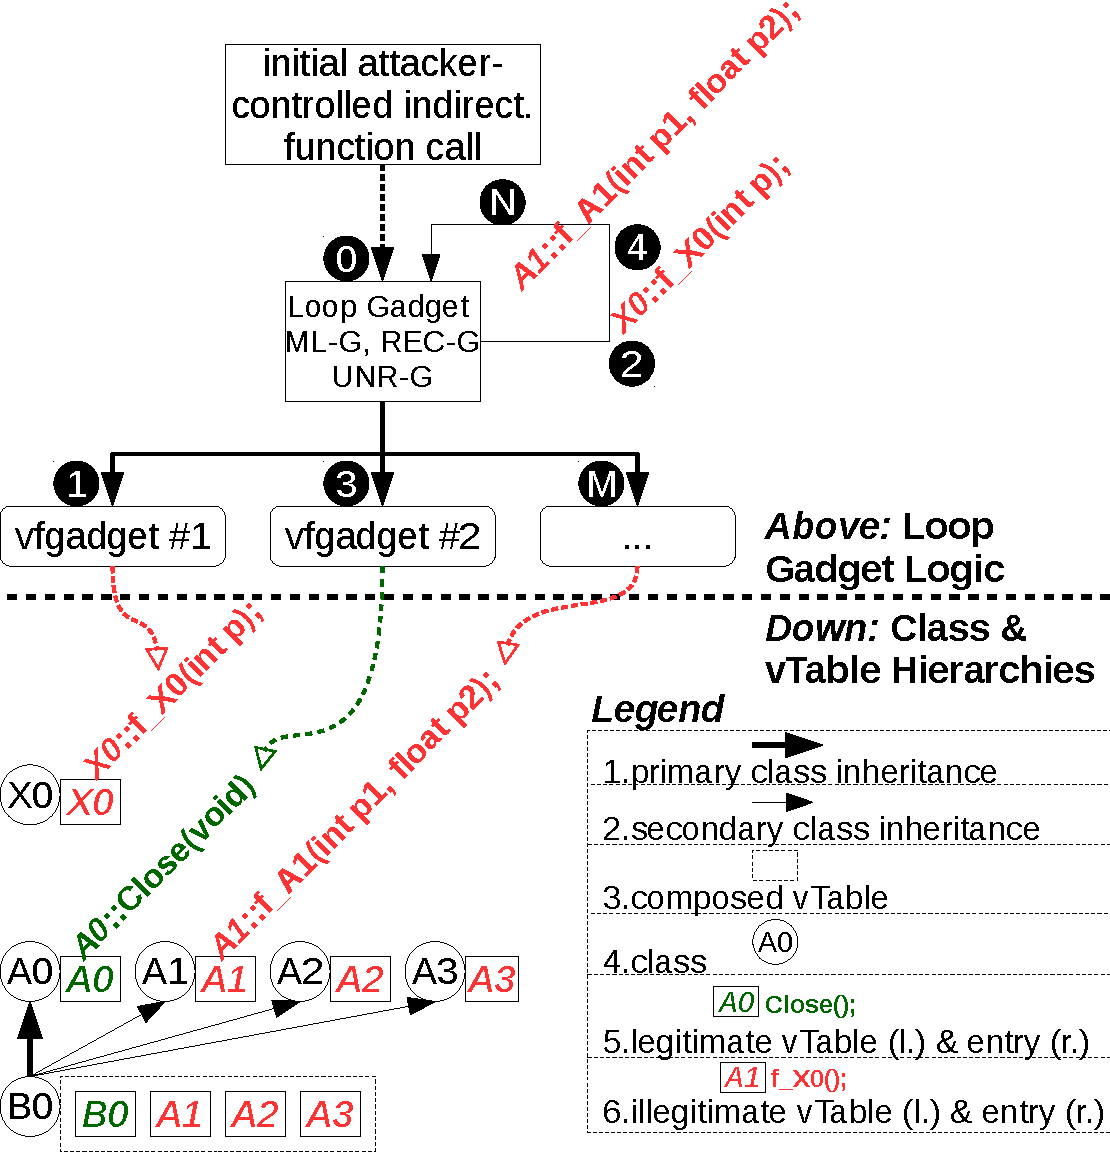
\includegraphics[width=.22\textwidth]{figures/loop.pdf}}
%      \put(.031, 2.5){\usebox{\firstlisting}}
%    \end{picture}}
% \vspace{-2.6cm}
% % \caption{Description of how a counterfeit object-oriented programming main loop gadget (ML-G) works.}
% \caption{COOP loop gadget (ML-G, REC-G, UNR-G) at work.}
% \label{Code example used to illustrate how a COOP loop gadget works}
% \end{figure}
% 
% Figure~\ref{Code example used to illustrate how a COOP loop gadget works}
% depicts a C++ code example (left) and how a COOP main-loop gadget (right) 
% (\textit{i.e.,} based either on ML-G (main-loop) or REC-G (recursive-gadget) or UNR-G (unrolled COOP gadget), 
% see~\cite{crane:readactor++} for more details) is used to sequentially call COOP gadgets by iterating trough 
% a loop (REC-G excluded) controlled by the attacker.
% 
% First, the object dispatch (see Figure~\ref{Code example used to illustrate how a COOP loop gadget works} line 17) is exploited by the attacker
% in order to call different functions in the whole program by iterating on an array of fake objects previously inserted in the array.
% 
% Second, in order to achieve this the attacker previously exploits an existing program memory corruption (\textit{e.g.,} buffer overflow) 
% which is further used to corrupt an object dispatch, \ding{182}, by inserting fake objects in the array and by changing the number of initial loop iterations.
% Next she invokes gadgets, \ding{182} and \ding{184} up to {\tiny\encircle{\Large{M}}}, 
% through the calls, \ding{183} and \ding{185} up to {\tiny\encircle{\Large{N}}}, contained in the loop. 
% As it can be observed in Figure~\ref{Code example used to illustrate how a COOP loop gadget works} she 
% can invoke from the same callsite legitimate functions (in total {\tiny\encircle{\Large{N}}}) residing in the virtual table (vTable) inheritance path
% (\textit{i.e.,} at the time of writing this paper this type of information is particularly hard to recuperate from program binaries)
% for this particular callsite, indicated with green color vTable entries. 
% However, a real COOP attack invokes illegitimate vTable entries residing in the whole initial program class hierarchy (or the extended one)
% with less or no relationship to the initial callsite,
% indicated with red-color vTable entries.
% 
% Third, in this way different addresses contained in the program (1) (vTable) hierarchy (contains only virtual members), 
% (2) class hierarchy (contains both virtual and non-virtual members) and (or) the whole program address space can be called. 
% For example the attacker can call in any entry in the:
% (1) class hierarchy of the whole program,
% (2) class hierarchy containing only legitimate targets for this callsite,
% (3) virtual table hierarchy of the whole program,
% (4) virtual table hierarchy containing only legitimate targets for this callsite,
% (5) virtual table hierarchy and class hierarchy containing only legitimate targets for this callsite, and
% (6) virtual table hierarchy and class hierarchy of the whole program.
% 
% Finally, because there are no intrinsic language semantics---such as object cast checks---in the C++ programming language for object dispatches
% the loop gadget indicated in Figure~\ref{Code example used to illustrate how a COOP loop gadget works} can be unconstrained used to call 
% any possible entry in the whole program. Thus, making any program address a gadget part.
% 
% \subsubsection{Security Implications of Indirect Calls}
% % \textbf{Security Implications of Forbidden Indirect Calls.}
% \label{Security Implications of Forbidden Forward Indirect Calls}
% The C++ language standard (N3690~\cite{iso:iecN3690}) does not specify what happens when calling different virtual table entries from an indirect callsite. 
% The standard says that we have a virtual function-related undefined behavior when: (citation) \textit{a virtual function call uses an explicit class member access and 
% the object expression refers to the complete object of x or one of that object's base class sub-objects but not x or one of its base class sub-objects}. As 
% undefined behavior is not a clearly defined concept, we argue that in order to be able to deal with undefined or unspecified behavior related to 
% virtual function calls one needs to know how these language-dependent concepts are implemented inside the used compilers.
% 
% Forbidden forward-edge indirect calls are the result of a vPointer corruption. A vPointer corruption is not a vulnerability, but rather a capability which
% can be the result of a spatial or temporal memory corruption triggered by: 
% (1) bad-casting~\cite{byoungyoung:typecasting} of C++ objects, 
% (2) buffer overflow in a buffer adjacent to a C++ object or 
% (3) a use-after-free condition~\cite{schuster:coop}.
% A vPointer corruption can be exploited in several ways. A manipulated vPointer can be exploited by pointing it in any existing or added program virtual 
% table entry or into a fake virtual table which was added by an attacker. For example in case a vPointer
% was corrupted than the attacker could highjack the control flow of the program and start a COOP attack~\cite{schuster:coop}.
% 
% vPointer corruptions are a real security threat which can be exploited if there is a memory corruption (\textit{e.g.,} buffer overflow) which is adjacent 
% to the C++ object or a use-after-free condition. As a consequence, each corruption which can reach an object (\textit{e.g.,} bad object casts) is a potential
% exploit vector for a vPointer corruption. Interestingly to notice in this context is that through:
% (1) memory layout analysis (through highly configurable compiler tool chains) of source code based locations which are highly prone to memory corruptions such 
% as declarations and uses of buffers, integers or pointer deallocations one can obtain the internal machine code layout representation;
% (2) analysis of a code corruption which is adjacent (based on (1)) to a C++ object based on application class hierarchy, the virtual table hierarchy and each
% location in source code where an object is declared and used (\textit{e.g.,} modern compiler tool chains can spill out this information for free), one can 
% derive an analysis which can determine---up to a certain extent---if a memory corruption can influence (\textit{e.g.,} is adjacent to) a C++ object.
% 
% Finally, tools based on these two concepts (\textit{i.e.,} (1) and (2)) can be used by attackers, \textit{e.g.,} to find new vulnerabilities, and by defenders
% to harden the source code only at the places which are most exposed to such vulnerabilities (\textit{i.e.,} targeted security hardening).
% 
% \subsection{Real COOP Attack Example}
% \label{Real COOP Attack Example}
% % \textbf{Real COOP Attack Example.}
% The bug CVE-2014-3176 was exploited by Crane \textit{et al.}~\cite{crane:readactor++} in order to perform a
% COOP attack, on the Google Chromium Web browser. The details of this attack are highly complex involving not properly 
% handled interaction of browser extensions between the IPC, the sync API, and Google V8 engine and for this reason we briefly present a better
% documented COOP exploit which is in principle similar with this attack.
% 
% \label{Running Example: CVE X}
% %%second pic
% \begin{figure}[h!]
%     \centering
%     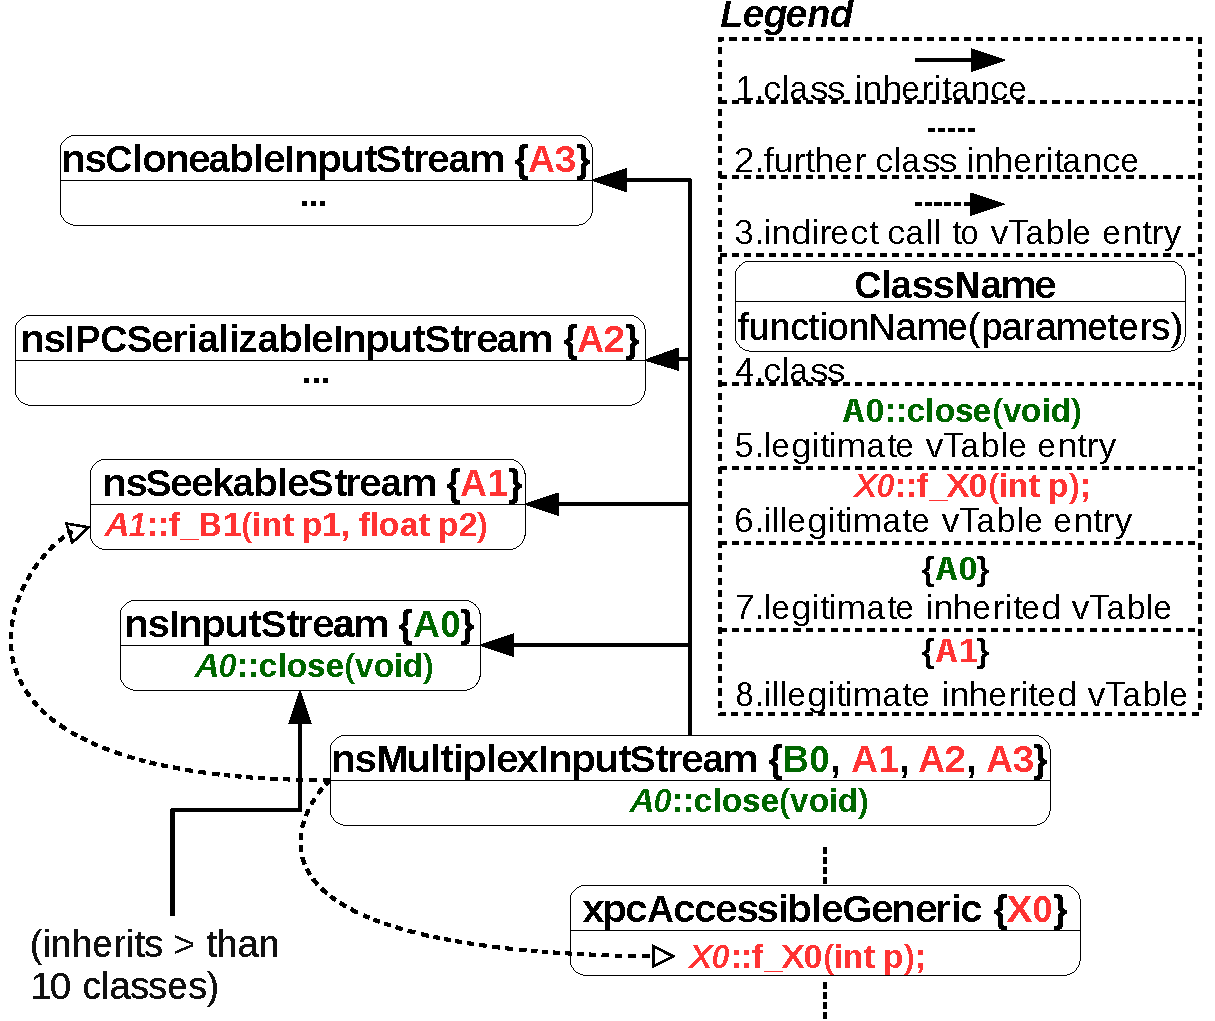
\includegraphics[width=0.35\textwidth]{figures/class_hierarchy.pdf}
% \caption{Class hierarchy of classes used in the COOP attack.}
% \label{Class exploit}
% \vspace{-.29cm}
% \end{figure}
% Figure~\ref{Class exploit} depicts~\footnote{The class inheritance hierarchy of the classes involved in the COOP attack against the Firefox browser. Red letters 
% indicate forbidden virtual table entries and green letters indicate allowed virtual table entries for the given indirect callsite
% contained in the main loop gadget.} a turing complete COOP attack~\cite{schuster:coop} which was used to attack the Mozilla Firefox Web browser. 
% By exploiting an existing buffer overflow bug the attacker was able to call into existing virtual table entries by having a main loop gadget at his disposal.
% 
% First, the attacker uses the C++ class \texttt{nsMultiplexInputStream} (see Figure~\ref{Class exploit}) which contains a 
% main loop gadget (ML-G) inside the \texttt{nsMultiplexInputStream::Close(void)} 
% function in order to perform indirect calls by dispatching calls on the fake objects contained in the array. The objects 
% contained in the array during normal execution are of \texttt{nsInputStream} type and each of the objects will call the 
% \texttt{Close(void)} function in order to close each of the previously opened streams. 
% 
% Second, for performing the COOP attack, the 
% attacker crafts a C++ program containing an array buffer holding six fake objects. These fake objects can call inside (and outside) 
% the initial class and virtual table hierarchies with no constraints. During the attack a buffer is created in order to hold the 
% fake objects. The crafted buffer will be used instead of the real code in order to call different functions available in the program code. 
% For example, the attacker calls a function contained in the class \texttt{xpcAccessibleGeneric} which is not in the class 
% hierarchy or virtual table hierarchy of the initially intended type of objects used inside the array. Moreover, the header 
% file of this class (\texttt{xpcAccessibleGeneric}) is not included in the class \texttt{nsMultiplex-InputStream}. 
% 
% Third, in total six fake objects are used to call into functions residing in unrelated class hierarchies with varying number of parameters 
% and return types. The final goal of this attack is to prepare the program memory such that a Unix shell can be opened at 
% the end of this attack.
% 
% 
% Finally, this example illustrates why detecting vPointer corruptions is not trivial for real-world applications. As depicted in 
% Figure~\ref{Class exploit}, the class \texttt{nsInputStream} has 11 classes which inherit directly or indirectly from 
% this class. The classes \texttt{nsSeekableStream}, \texttt{nsIPCSerializableInputStream} and \texttt{nsCloneableInputStream}
% provide additional inherited virtual tables which represent illegitimate calltargets for the initial \texttt{nsInputStream} 
% objects and legitimate calltargets for the six fake objects which were added during the attack. Furthermore, declaration and
% usage of the objects can be widely spread out in the source code. This makes detection of the object types 
% (\textit{i.e.,} base class), range of virtual tables (\textit{i.e.,} longest virtual table inheritance path for a
% particular callsite) and parameter types of the virtual table entries (\textit{i.e.,} functions) in which it is 
% allowed to call a trivial task for source code applications, but a hard task when one wants to apply similar 
% security policies (\textit{e.g.,} which rely on parameter types of virtual table entries) to binary executables.

\subsection{Checking Indirect Calls in Practice}
% \textbf{Checking Indirect Forward-Edge Calls in Practice.}
\label{C++ Indirect Calls in Practice}
To the best of our knowledge, only the IFCC/VTV~\cite{vtv:tice} compiler based tools (up to 8.7\% performance overhead) are deployed in practice
and can be used to check legitimate from illegitimate indirect forward-edge calls during runtime. Virtual pointers are checked based on the class hierarchy. 
Furthermore, ShrinkWrap~\cite{haller:shrinkwrap} (to the best of our knowledge not deployed in practice) is a tool which further reduces the legitimate 
virtual table ranges for a given indirect callsite through precise analysis of the program class hierarchy and virtual table hierarchy. Evaluation results
show similar performance overhead but more precision with respect to legitimate virtual table entries per callsite. We noticed by analyzing the previous 
research results that the overhead incurred by these security checks can be very high due to the fact that for each callsite many range checks have to be
performed during runtime. Therefore, in our opinion, despite its security benefit these types of checks cannot be applied to high performance applications.

A number of other highly promising tools (albeit also not deployed in practice) can overcome some of the drawbacks of the previously described tools. 
Bounov \textit{et al.}~\cite{bounov:interleaving} presented a tool ($\approx$1\% runtime overhead)
for indirect forward-edge callsite checking based on virtual table layout interleaving. The tool has better performance than VTV and better precision with
respect to allowed virtual tables per indirect callsite. Its precision (selecting legitimate virtual tables for each callsite) compared to ShrinkWrap is
lower since it does not consider virtual table inheritance paths. vTrust~\cite{zhang:vtrust} (average runtime overhead 2.2\%) enforces two layers of defense
(virtual function type enforcement and virtual table pointer sanitization) against virtual table corruption, injection and reuse. TypeArmor~\cite{veen:typearmor}
(around 3\% runtime overhead) enforces a CFI-policy based on runtime checking of caller/callee pairs and function parameter count matching. It is important to note 
that there are no C++ language semantics which can be used to enforce type and parameter count matching for indirect caller/callee pairs, this could be addressed
with specifically intended language constructs in the future.



